%!TEX program = xelatex
\documentclass[9pt,dvipsnames,table]{beamer}
\usepackage[no-math,cm-default]{fontspec}
%\usepackage[indentfirst]{xeCJK}
\usepackage{amsmath}
\usepackage{amsthm}
\usepackage{amssymb}
\usepackage{verbatim}
\usepackage{indentfirst}
\usepackage{syntonly}
\usepackage{beamerthemesplit}
\usepackage{euler}
\usepackage{ulem}
\usepackage{listings}
\usepackage{etoolbox}
\usepackage{zhspacing}
\usepackage{url}
%\usepackage{paralist}

\defaultfontfeatures{Mapping=tex-text}
\zhspacing
\renewcommand{\skipzh}{\hskip 0.02em plus 0.2em minus 0.1em}
\renewcommand{\skipenzh}{\hskip 0.1em plus 0.15em minus 0.05em}
\newfontfamily{\zhfont}[BoldFont=Adobe Heiti Std, ItalicFont=Adobe Kaiti Std]{Adobe Song Std}
\setmonofont[Scale=1]{Consolas}

\usetheme{Berlin}
\usecolortheme{beaver}
%\usefonttheme[onlymath]{serif}
\usefonttheme{professionalfonts}
\setbeamerfont{section in toc}{size=\fontsize{10pt}{\baselineskip}}

\newcommand{\hlink}[1]{
	\footnote{\fontsize{6pt}{\baselineskip}\href{#1}{\textsl{\underline{\url{#1}}}}}
}
\newcommand{\graph}[2]
{\noindent
\begin{figure}[h!]
	\centering
	\includegraphics[width=#2 \textwidth]{image/#1}
\end{figure}}

\lstset{language=C++,
	extendedchars=false,
	basicstyle=\ttfamily\footnotesize,
	keywordstyle=\bfseries\color{blue},
	identifierstyle=\color{blue!60!black},
	commentstyle=\itshape\color{gray},
	escapeinside=`'}

%\let\enumerate\compactenum
%\let\endenumerate\endcompactenum
%\let\itemize\compactitem
%\let\enditemize\endcompactitem
%\setlength{\plparsep}{0em}
%\setlength{\plitemsep}{0.2em}
%\setlength{\pltopsep}{0.2em}
\setlength{\parindent}{2em}
\setlength{\parskip}{0.25em}
\setlength{\footskip}{30pt}
\setlength{\baselineskip}{1.2\baselineskip}
\renewcommand\arraystretch{1.2}

\setbeamercolor{math text}{fg=black}
\setbeamertemplate{qed symbol}{ $ \square $ }
\setbeamerfont{headline}{size=\fontsize{7.5pt}{\baselineskip}}
\setbeamerfont{footline}{size=\fontsize{7.5pt}{\baselineskip}}
\setbeamertemplate{theorems}[numbered]
\renewcommand{\thetheorem}{\arabic{subsubsection}.\arabic{theorem}}
\renewcommand{\thelemma}{\arabic{subsubsection}.\arabic{lemma}}
\newenvironment{qedframe}{%
	\begin{frame}[environment=qedqedframe]%
	}{%
	\qed
	\end{frame}%
}
\renewcommand{\appendixname}{结语}

\makeatletter
\patchcmd{\beamer@sectionintoc}{\vskip 1.5em}{\vskip 1em}{}{}
\makeatother

\begin{document}

\title[动态规划例题选讲]{\fontsize{24pt}{\baselineskip}\textbf{动态规划例题选讲}}
\subtitle[]{\fontsize{16pt}{\baselineskip}Dynamic Programming by Examples}
\author{清华大学计算机系~~胡泽聪}
%\institute[清华大学计算机系~~胡泽聪]{}
\date{}

\maketitle

%\setcounter{tocdepth}{1}
\begin{frame}
	\frametitle{目录}
	\tableofcontents[hideallsubsections]
\end{frame}

\section{前言}
\subsection{}
\begin{qedframe}
	\frametitle{关于我}
	\begin{itemize}
		\item 高中:湖南师大附中
		\item NOI2013 Au
		\item 现就读于THU计算机系
	\end{itemize}
\end{qedframe}
\begin{qedframe}
	\frametitle{关于课程}
	通过例题学习动态规划。 \pause
	\vskip 1em
	动态规划与其他知识点的区别:
	\begin{itemize}
		\item 网络流
		\item 数据结构
	\end{itemize}
\end{qedframe}

\section{Part I}

\subsection{CodeChef JUNE13 LEMOUSE}
\begin{qedframe}
	\frametitle{Little Elephant and Mouses\hlink{https://www.codechef.com/JUNE13/problems/LEMOUSE}}
	有一个$n\times m$的网格。有一头大象,初始时在$(1,1)$,要移动到$(n,m)$,每次只能向右或者向下走。有些格子中有老鼠,如果大象所在的格子和某个有老鼠的格子的曼哈顿距离$\leq1$,大象就会被那只老鼠吓到。
	
	求一条移动路径,使得吓到过大象的老鼠数量最少。$n,m\leq100$。
\end{qedframe}
\begin{qedframe}
	\frametitle{Little Elephant and Mouses}
	如果多次经过一只老鼠旁边也会被吓多次,直接DP就好了。而这里只会被吓一次,我们需要往状态中加点东西。\pause
	
	注意到,一只老鼠最多能影响我们三步,因此只要记录上一步的走法即可。转移时分情况讨论。 
\end{qedframe}

\subsection{Codeforces Round \#198 (Div. 1): Problem C}
\begin{qedframe}
	\frametitle{Iahub and Permutations\hlink{http://codeforces.com/contest/341/problem/C}}
	有一个长度为$n$的排列$a$,其中有一些位置被替换成了$-1$。你需要尝试恢复这个排列,将$-1$替换回数字。
	
	求有多少种可行的替换方法,满足得到的是一个排列,且不存在$a_i=i$的位置。$n\leq 2000$。
\end{qedframe}
\begin{qedframe}
	\frametitle{Iahub and Permutations}
	我们用一个$n\times n$的棋盘来表示一个排列,第$i$行第$j$列如果被标记,则代表数字$i$填在了第$j$个位置($a_j=i$)。对于给定的排列,不为$-1$的位置已经被标记在棋盘上,而棋盘的主对角线上($a_i=i$)不可以被标记。\pause
	
	从棋盘中删去不为$-1$的位置的列,以及已经出现了的数字的行,记此时棋盘大小为$N$。不难发现,每列不可被标记的位置至多只有1个,每行也是同样。记这种位置的数量为$M$。\pause
	
	令$f[N,M]$表示,在这样的棋盘上标记$N$个格子的方案数。转移方程为:
	\[ f[n,m]=f[n,m-1]-f[n-1,m-1] \]
	边界为$f[i,0]=i!$。
	
	转移方程的含义为,相比起$f[n,m-1]$的状态,$f[n,m]$的状态要多一个不可标记的位置,而标记了这个位置的方案数为$f[n-1,m-1]$,因此从中减去。
\end{qedframe}

\subsection{TopCoder Open 2014 Round 1B L3}
\begin{qedframe}
	\frametitle{EagleInZoo\hlink{https://community.topcoder.com/stat?c=problem_statement&pm=13117}}
	有一棵$n$个节点的有根树。现在依次飞来了$k$只鹰,想在树上休息。每只鹰初始都在根节点,然后采取如下操作:
	\begin{enumerate}
		\item 如果当前所在的节点是空的,那么占据这个节点休息;
		\item 否则,如果该节点有儿子节点,那么等概率随机飞到一个儿子节点上;
		\item 否则,这只鹰会放弃休息,直接飞走。
	\end{enumerate}
	
	求第$k$只鹰最后留在树上的概率。$n\leq 50$,$k\leq 100$。
\end{qedframe}
\begin{qedframe}
	\frametitle{EagleInZoo}
	首先注意到,这个问题有明显的子结构:当鹰飞到子树的树根时,整个问题和鹰初始时在根节点是一样的。\pause
	
	因此我们直接令$p[x,k]$代表第$k$只鹰从节点$x$出发,最后能留在树上的概率。记节点$x$的儿子个数为$c_x$,边界情况有:
	\begin{itemize}
		\item $p[x,1]=1$;
		\item 如果$c_x=0$,那么对于$k>1$都有$p[x,k]=0$。
	\end{itemize}
\end{qedframe}
\begin{qedframe}
	\frametitle{EagleInZoo}
	而对于一般情况,有下面的公式:
	\[ p[x,k] = \sum_{y\in\mathrm{child}(x)}\frac{1}{c_x}\sum_{i=0}^{k-2}\binom{k-2}{i}\left(\frac{1}{c_x}\right)^i\left(1-\frac{1}{c_x}\right)^{k-2-i}p[y,i+1] \]
	
	我们这么理解:第一只鹰必然落在节点$x$上,假设第$k$只鹰最后落在$x$的儿子$y$的子树内,我们考虑有几只鹰也曾飞进了这棵子树。如果是$i$只,那么概率为$\binom{k-2}{i}\left(\frac{1}{c_x}\right)^i\left(1-\frac{1}{c_x}\right)^{k-2-i}$。
	
	复杂度为$O(nk^2)$。
\end{qedframe}

\subsection{CodeChef APRIL14 ANUCBC}
\begin{qedframe}
	\frametitle{Cards, bags and coins\hlink{https://www.codechef.com/APRIL14/problems/ANUCBC}}
	$n$个数字,选出其一个子集。
	
	求有多少子集满足其中数字之和是$m$的倍数。$n\leq 100000$,$m\leq 100$,最多90组数据。
\end{qedframe}
\begin{qedframe}
	\frametitle{Cards, bags and coins}
	有个显然的背包做法……只是会TLE。\pause
	
	注意到$m$只有100,也就是说可以当做有$m$种物品的多重背包做。求最大值的话可以用二进制拆分的方法,但求方案数不行。\pause
	
	我们依次考虑每个物品,令$g_i$为选出一些这个物品使得体积对$m$取模为$i$的方案数,这个就等于一些组合数之和。
	
	那么现在又相当于$m$个物品了,做一遍背包即可。复杂度为$O(n+m^3)$。
\end{qedframe}

\section{Part II}

\subsection{CodeChef FEB14 LEMOVIE}
\begin{qedframe}
	\frametitle{Little Elephant and Movies\hlink{https://www.codechef.com/FEB14/problems/LEMOVIE}}
	对于一个序列,定义其``激动值''为序列中严格大于前面所有数的元素的个数。比如,$\{1,1,5,6,5\}$的激动值为$3$。
	
	给定$n$个数$p_1,p_2,\ldots,p_n$,求这$n$个数的所有排列中,激动值不超过$k$的个数。$1\leq k\leq n\leq 200$,$1\leq p_i\leq200$。
\end{qedframe}
\begin{qedframe}
	\frametitle{Little Elephant and Movies}
	先记录相同的数的个数,然后去重。\pause

	从大到小考虑每组相同的数。令$f[i,j]$代表已经插入前$i$大的数,且激动值为$j$的序列方案数。\pause

	考虑当前这组数插入在哪些位置。每一组数的贡献至多为$1$,有贡献当且仅当至少一个数被插在了最前面。无论插入在什么位置,已有的激动值不会减少。 \pause

	假设已经插入了$x$个数,当前这组有$y$个数,没有一个数被插在最前面的方案数为
	\[y!\binom{x+y-1}{x-1}\]
	至少一个被插在最前面的可以类似算。

	复杂度$O(nk)$。
\end{qedframe}
\begin{qedframe}
	\frametitle{Little Elephant and Movies}
	如果激动值的定义为,序列中相邻的且构成逆序对的数对呢?
	
	(为啥会有这个问题,是因为我最开始就把题目看成这个了)\pause
	\vskip 1em
	这个问题实际上稍难于原问题。

	做法类似。从小到大考虑,此时插入一个数可能会抵消之前的激动值。枚举有几个数插在原来的非逆序对之间,可以类似地算出方案数。
	
	复杂度$O(nk^2)$。
\end{qedframe}

\subsection{Codeforces Round \#221 (Div. 1): Problem C}
\begin{qedframe}
	\frametitle{Circling Round Treasures\hlink{http://codeforces.com/contest/375/problem/C}}
	在一个$n\times m$的地图上,有一些障碍,还有$a$个宝箱和$b$个炸弹。你从$(sx,sy)$出发,走四连通的格子。你需要走一条闭合的路径,可以自交,且围出来的复杂多边形内不能包含任何炸弹。你围出来的复杂多边形中包含的宝箱的价值和就是你的收益。
	
	求最大收益。$n,m\leq 20$,$a+b\leq 8$。
	
	\graph{CF221.png}{0.25}
\end{qedframe}
\begin{qedframe}
	\frametitle{Circling Round Treasures}
	先考虑这个问题:如何判断一个点是否被复杂多边形所包含(不考虑在边上)?\pause
	\vskip 1em
	\textbf{射线法}。找一条由该点发出且不经过多边形上点的射线,然后看这条射线与多边形交了几次。如果交了奇数次,则在多边形内,否则在多边形外。
	\vskip 1em
	是否可以把这一方法用到这道题中?
\end{qedframe}
\begin{qedframe}
	\frametitle{Circling Round Treasures}
	其实是可以的。我们对于每个宝箱和炸弹维护一条射线,然后维护这些射线中哪些穿过了路径奇数次。 \pause
	
	令$F[x,y,k]$表示,当前在$(x,y)$,且集合$k$中的射线穿过了路径奇数次,这样的状态是否可行。
	
	转移时枚举下一步,然后看两步之间的线段穿过了哪些射线,并更新集合$k$。
	
	最后枚举所有集合$k$,要求炸弹的射线穿过路径偶数次,且$F[sx,sy,k]=\ $\texttt{true}。用集合中宝箱的价值和更新答案。
	
	复杂度$O(nm(a+b)2^{a+b})$。
\end{qedframe}

\subsection{<Source Unknown>}
\begin{qedframe}
	\frametitle{Parallel}
	给定一个有$N$个点的图,每个点都向外连出一条有向边,边长均为1。现要求在图中添加尽量少的从1号点出发的边,使得1号节点到每个节点的距离都不超过$K$。
	
	求添加的最少边数。$N\leq 100000$。
\end{qedframe}
\begin{qedframe}
	\frametitle{Parallel}
	不难发现,这个图是一个环套树。从1号点向某个节点连边就相当于把那个节点的距离设为1。\pause
	
	一个显然的结论是,我们需要对每个入度为0的节点添加一条边,因为不然这些节点根本不能从1号点到达。而对于树的部分,我们可以使用自底向上的树形DP简单处理。问题在于环的部分。
\end{qedframe}
\begin{qedframe}
	\frametitle{Parallel}
	一个朴素的$O(N^2)$的处理环的方法是枚举断开的地方(即把环视为从某个节点开始的链),然后按照在树上的方法$O(N)$做一遍,取所有断开处答案的最小值。\pause
	
	可以发现,对于环上每一个距离超过$K$的点,在该点的前$K-1$个点或该点之中至少存在一个点要从1连边。那么我们只需要断开$K$个地方。\pause
	
	同时我们可以处理出数组$D[i]$,表示链上的$i$号点之后最近的距离大于$K$的点的编号,如果$i$号点本身的距离就大于$K$,则$D[i]=i$。这样我们访问完$x$号点时,就可以直接访问$D[x]$,而不用每次访问下一个节点了;而更新到一个需要连边的点之后,只需要往后跳$K$个节点再访问$D$数组即可。
	
	这样在环上做一遍的复杂度就是$O(N/K)$的了,总的复杂度也就变成了$O(K\cdot N/K = N)$。
\end{qedframe}

\subsection{HNOI2006 D1P4}
\begin{qedframe}
	\frametitle{Pandora\hlink{http://www.lydsy.com/JudgeOnline/problem.php?id=1194}}
	$k$个DFA,选出尽量多的自动机$a_0,a_1,a_2,\ldots,a_t$,使得$a_1$包含$a_0$、$a_2$包含$a_1$,以此类推。$k\leq 50$。
	
	DFA的字符集为$\{0,1\}$,节点数$n\leq 50$。
\end{qedframe}
\begin{qedframe}
	\frametitle{Pandora}
	请先听我口头介绍什么是DFA。\pause
	
	用二元组$(x,y)$表示当前状态处在A的$x$点与B的$y$点上,初始为$(0,0)$。转移时$x$和$y$一起走到加0和加1后的位置,即$(px0,py0)$和$(px1,py1)$,如果已经访问过该状态就不转移。假设在某个状态中$x$为输出元而$y$不是,那么B就不能输出这个A能输出的字符串,即B不包含A。如果不存在这种状态,则B包含A。\pause
	
	用上面的方法对每两个自动机都进行判断然后建图。建完之后缩强连通分量,得到的会是一个拓扑图。在这个拓扑图上DP即可。
\end{qedframe}

\section{Part III}

\subsection{TopCoder SRM472 D1L2}
\begin{qedframe}
	\frametitle{TwoSidedCards\hlink{https://community.topcoder.com/stat?c=problem_statement&pm=10947}}
	有$N$张牌,正反都有数字。所有正面和所有反面的数字各构成一个排列。将牌排成一排,每张牌可以正面朝上或者反面朝上,这样可以构成一个序列。
	
	给定$N$张牌正面和反面的数字,求:所有可能的序列方案数。$N \leq 50$。
	\vskip 1em
	比如:3张牌,正面分别为1、2、3,反面分别为1、3、2。那么一共有12种序列:
	\begin{center}
	123、132、213、231、312、321、
	
	133、313、331、122、212、221。
	\end{center}
\end{qedframe}
\begin{qedframe}
	\frametitle{TwoSidedCards}
	假设$N$足够小,可以让我们枚举哪些牌正面朝上。
	
	那么可以发现,可能会有一些数字重复出现,而且重复出现次数最多为2。
	
	记重复出现的数字个数为$k$,那么根据多重集的排列公式,这些牌的不同排列数为:
	\[\frac{N!}{2^k}\]
	
	不妨枚举$k$。现在我们要求的就是,对于任意合法的$k$,在多少种牌的正反方案中有$k$个数出现了2次。
\end{qedframe}
\begin{qedframe}
	\frametitle{TwoSidedCards}
	我们把所有牌按正面数值$1\sim N$的顺序摆成一排。
	
	这样我们就可以把反面数值视为一个置换,把这张牌翻面就相当于置换这一个位置。
	
	可以发现,置换的不同循环之间是不影响的。
	
	现在我们就来考虑一个循环。记这个循环的长度为$L$,显然有$k\leq\lfloor L/2\rfloor$。
\end{qedframe}
\begin{qedframe}
	\frametitle{TwoSidedCards}
	建立图论模型。
	
	将每张牌正面的数字视为一个节点,连向其反面数字对应的节点。
	
	可以发现,整张图会是若干个环,一个循环就对应图中的一个环。
	
	有了这张图我们可以干什么呢?
\end{qedframe}
\begin{qedframe}
	\frametitle{TwoSidedCards}
	一张牌可以视为图中的一条有向边,从其正面的数字指向反面的数字。如果将牌翻面,就相当于将边反向。
	
	出现两次的数也即入度为2的节点,这样的节点的一定是和入度为0的节点个数相等的,而且在同一个环上交替出现。\pause
	
	由此可以得到公式:长度为$L$的循环中有$k$个数出现两次时,牌的正反的方案数为
	\[ 2\cdot\binom{L}{2k} \]
	即从$L$个数字中各选出$k$个作为出现2次和0次的,而这$2k$个数内部有2种方案(第一个数出现2次还是0次)。
	
	特别地,$k=0$时方案数为1(无论全部正面还是反面,朝上的数的集合相同)。
\end{qedframe}
\begin{qedframe}
	\frametitle{TwoSidedCards}
	不过刚才只考虑了一个循环内牌的正反,如何回到原问题?\pause
	\vskip 1em
	用背包求出对于整个序列出现两次的数为$k$个的方案数。最后用最开始的公式计算排列即可。
\end{qedframe}

\subsection{TopCoder SRM570 D1L2}
\begin{qedframe}
	\frametitle{CentaurCompany\hlink{https://community.topcoder.com/stat?c=problem_statement&pm=12428}}
	$n$个节点的树,每个节点被随机染成黑白两色之一。现在要使同种颜色的点连通,因此需要加边。每个节点最多免费加一条边,如果还要再加,那么每加一条边都需要付出1的代价(注意是针对节点而言的)。
	
	求期望最小代价。$n\leq 36$。
\end{qedframe}
\begin{qedframe}
	\frametitle{CentaurCompany}
	先考虑单个的问题:给定一种染色方案,如何求其最小代价?\pause
	
	对于染成同一种颜色的$n$个点,如果它们分布在$c$个连通块中,那么产生的费用为$\max(0,2c-n-2)$。\pause
	
	那么令$f[col,p,n_1,c_1,n_2,c_2]$代表$p$的颜色为$col$,而且以$p$为根的子树中被染上颜色1和2的点有$n_1$和$n_2$个,分成$c_1$和$c_2$个连通块,这样的状态的个数。注意$n_1+n_2=size[p]$,因此状态数为$O(n^4)$。\pause
	
	转移时枚举儿子颜色,如果儿子的颜色和父亲相同则不产生新的连通块,否则会产生一个新的连通块。再枚举儿子子树中颜色1的点数,用类似背包的方法求解。转移复杂度为$O(n^3)$。
	
	总复杂度高达$O(n^7)$,需要优化。
\end{qedframe}
\begin{qedframe}
	\frametitle{CentaurCompany}
	优化其实也很简单,注意到计算答案只需要$2c_1-n_1$和$2c_2-n_2$的值,因此我们直接维护它。\pause
	
	再进一步,由期望的线性性,我们知道
	\[E((2c_1-n_1) + (2c_2-n_2)) = E(2c_1-n_1) + E(2c_2-n_2)\]而由于对称性,这两个东西是相等的。因此我们只要知道一个颜色的$2c-n$即可,复杂度优化到$O(n^3)$。
\end{qedframe}

\subsection{TopCoder SRM489 D1L3}
\begin{qedframe}
	\frametitle{AppleTrees\hlink{https://community.topcoder.com/stat?c=problem_statement&pm=11213}}
	一排$D$个坑中要种下$n$棵树,每棵树有半径$r_i$,表示其左右$r_i$的范围内不能种其他树。
	
	求合法的方案数。$D \leq 100000$,$n,r_i\leq 40$。
\end{qedframe}
\begin{qedframe}
	\frametitle{AppleTrees}
	假设我们已经知道树的相对顺序,我们可以先把它们尽量紧凑地排在一起,然后在树之间插入空的坑。\pause

	如何计算给定顺序时,两端的两棵树之间的最短距离?\pause 相邻两棵树的距离为这两棵树半径的较大值。\pause
	\vskip 1em
	我们考虑按某种顺序一棵一棵种下这些树。比如按照$r_i$从小到大。

	一个问题是,只有当我们确定两棵树之间不会再插入新的树的时候,我们才能确定这两棵树之间的距离是多少。
\end{qedframe}
\begin{qedframe}
	\frametitle{AppleTrees}
	那么在状态中记录:目前两端的两棵树之间的距离$k$,以及还有多少对相邻的树之间还会插入别的($r_i$更大的)树。称后者中满足条件的两棵树之间存在``缝隙''。

	当我们确定两棵树之间不会再有别的树的时候,我们才将其距离计入$k$。缝隙的距离不计入$k$。\pause
	\vskip 1em
	具体的DP方案如下:用$f[i,j,k]$表示:前$i$棵树目前有$j$个缝隙,最两端树之间的距离为$k$(不算缝隙)的方案数。
	
	转移时枚举下一棵树放哪:缝隙中还是两端,同时讨论新放的树与左右的树之间是否留缝隙。
	
	最终答案$\sum f[N,0,k]\times\binom{D-k+N}{D-k}$。复杂度$O(N^3r_i)$。
\end{qedframe}

\subsection{CodeChef May14 SEAGM}
\begin{qedframe}
	\frametitle{Sereja and Game\hlink{https://www.codechef.com/MAY14/problems/SEAGM}}
	$n$个数(可能存在相同的数),双方轮流取数。如果在一方选取之后,所有已选取数字的GCD变为1,则此方输。
	
	问:
	\begin{enumerate}
		\item 若双方均采取最优策略,先手是否必胜?
		\item 若双方随机取数,先手获胜的概率为多少?
	\end{enumerate}
	
	$n,a_i\leq100$。
\end{qedframe}
\begin{qedframe}
	\frametitle{Sereja and Game}
	令$f[i,j]$表示GCD为$i$,未选而且是$i$的倍数的数有$j$个的状态。\pause
	
	转移时,要么是转移到$f[i,j-1]$,要么是枚举一个令GCD减小的数转移。在GCD减小后,原来是倍数的还是倍数,此外还可能有之前不是倍数的,现在变成了倍数,统计一下即可。
	
	通过预处理倍数可以做到$O(n)$的转移。而两问都可以用这个方法解决。\pause
	\vskip 1em
	这个方法的核心在于找到了一个合理的考虑牌的顺序,使得我们能划分阶段。
\end{qedframe}

\section{Part IV}

\subsection{TopCoder SRM473 D1L3}
\begin{qedframe}
	\frametitle{RooksParty\hlink{https://community.topcoder.com/stat?c=problem_statement&pm=10980}}
	有$N$种颜色的车(国际象棋),每种$Col_i$个,放置在$R\times C$的棋盘上。如果有两个不同颜色的车处于同行或同列,它们就会互相攻击。

	求使得所有车不互相攻击的摆放方案数。$R,C\leq 30$,$N\leq 10$。
\end{qedframe}
\begin{qedframe}
	\frametitle{RooksParty}
	每行和每列的所有格子要么是同一种颜色的车,要么为空。那么给每行和每列标上一种颜色。
	
	一种颜色的车能放置的格子为,该行和该列的颜色都为车的颜色的格子。也即每种颜色之间无关。\pause
	\vskip 1em
	令$F[t,x,y]$表示颜色$1\sim t$的车占据$x$行和$y$列的方案数。
	\[ F[t,x,y] = \sum_{r=1}^{x}\sum_{c=1}^{y}F[t-1,x-r,y-c]\binom{x}{r}\binom{y}{c}S[Col_t,r,c] \]
	其中$S[n,r,c]$为将$n$个车摆放在$r\times c$的棋盘上,使得\textbf{每行每列都有至少一个车}的方案数(不考虑互相攻击,因为同色嘛)。
	
	公式很好理解:考虑当前颜色的车占据了哪几行哪几列,乘上摆放方案数,再递归考虑剩下的。
	
	注意边界和转移的合法性。
\end{qedframe}
\begin{qedframe}
	\frametitle{RooksParty}
	怎么求$S[n,r,c]$呢?\pause
	
	先只考虑列。令$R[n,r,c]$代表满足了每列有至少一个车的摆放方案数。\pause
	
	运用容斥原理:
	\[ R[n,r,c] = \sum_{i=0}^{c}(-1)^i\binom{c}{i}\binom{r(c-i)}{n} \]
	其中$i$代表有$i$列为空,和式的该项为有至少$i$列为空的摆放方案数。\pause
	
	在把行也加入考虑,类似可以得到:
	\[ S[n,r,c] = \sum_{j=0}^{r}(-1)^j\binom{r}{j}R[n,r-j,c] \]
	其中$j$代表有$j$行为空。
\end{qedframe}
\begin{qedframe}
	\frametitle{RooksParty}
	我们分析一下时间复杂度。
	\begin{itemize}
		\item 计算$f$的复杂度:状态$O(nRC)$,转移$O(RC)$,总复杂度$O(nR^2C^2)$。
		\item 计算$S$的复杂度:状态$O(Col_xRC)$,转移$O(R+C)$,总复杂度为$O(nRC(R+C))$。
	\end{itemize}
	
	算法的总复杂度为$O(nR^2C^2)$。
\end{qedframe}
\begin{qedframe}
	$S[n,r,c]$还有另外一种直接考虑二维问题的求法:
	\[ S[n,r,c] = \binom{r\cdot c}{n} - \sum_{i=1}^{r}\sum_{j=1}^{c}\binom{r}{i}\binom{c}{j}S[n,r-i,c-j] \]
	即从所有方案中减去有$i$行$j$列为空的方案。
	
	这个方法的复杂度为$O(nR^2C^2)$,可以稍作优化:
	\[ S[n,r,c] = \binom{r\cdot c}{n} - \sum_{i=1}^{r}\binom{r}{r-1}\sum_{j=1}^{c}\binom{c}{c-j}S[n,r-i,c-j] \]
	维护$G[k] = \sum_{j=1}^{c}\binom{c}{c-j}S[n,k,c-j]$,可以优化转移。总复杂度降为$O(nR^2C)$。
\end{qedframe}

\subsection{HNOI2015 D1P1}
\begin{qedframe}
	\frametitle{Arthur\hlink{http://www.lydsy.com/JudgeOnline/problem.php?id=4008}}
	玩家有一套共$n$张卡牌,每张卡牌都有一个技能。第$i$张卡牌的技能发动概率为$p_i\ (0<p_i<1)$,如果成功发动,则会对敌方造成$d_i$点伤害。

	一局游戏一共有$r$轮,在一轮中,系统将按照顺序依次考虑每张卡牌。对于一张卡牌,判定如下:
	\begin{enumerate}
		\item 如果这张卡牌已经发动过技能,则跳过之;
		\item 否则,设这张卡牌为第$i$张,那么其将以$p_i$的概率发动技能。如果技能发动,则对敌方造成$d_i$点伤害,并结束这一轮;
		\item 否则,考虑下一张卡牌。特别地,如果这张卡牌已经是最后一张(即第$n$张),则这一轮不发动技能,并结束这一轮。
	\end{enumerate}
	
	求出一局游戏中造成的伤害的期望值。$n\leq 220$,$r\leq 132$,最多444组测试数据。
\end{qedframe}
\begin{qedframe}
	\frametitle{Arthur}
	我们先来看一道简单的题:
	\begin{itemize}
		\item 求有多少$1\sim n$的排列,其逆序对数为$k$。\pause
	\end{itemize}
	\vskip 1em
	做法非常简单,令$f[i,j]$为$1\sim i$的排列中逆序对数为$j$的个数。\pause
	
	转移方程如下:
	\[ f[i,j] = \sum_{t=\max(1,j-i)}^{j}f[i-1,t] \]
	利用前缀和可以优化到$O(nk)$。
\end{qedframe}
\begin{qedframe}
	\frametitle{Arthur}
	设没有发动技能的一轮为``空轮''。

	我们可以把一种方案抽象为一个带空格的部分排列,空格为空轮,其他的为该轮发动的卡片。这样的抽象和原方案是一一对应的。\pause
	\vskip 1em
	先假设没有空轮。不妨考虑到最后发动了技能的卡片的集合,设为$S$。要求得到这一集合的概率,如果暴力做,应当枚举其所有排列。

	一个排列的概率即为,每轮的概率之积。而一轮的概率又是发动技能的卡片的$p_i$乘上$i$之前所有的$1-p_j$,再除去所有已发动卡片的$1-p_k$。\pause

	那么先不考虑已发动技能,之后再将其除去。设第$i$张卡牌在第$j$轮发动,那么对于第$j$轮之后发动的编号大于$i$的卡牌,都需要除一次$1-p_j$。为此,我们需要知道每个位置的顺序对数。
	
	直接套用开始的算法,按照$n\sim 1$的顺序枚举即可。复杂度为$O(nr^2)$。\pause
	
	进而,我们还可以直接在DP的时候选择集合。复杂度仍为$O(nr^2)$。
\end{qedframe}
\begin{qedframe}
	\frametitle{Arthur}
	如果考虑空轮呢?现在要处理的问题就是,确定了排列后,还需要向其中插入空格。同时一张卡片还需要对其之后的每个空格除一次$1-p_i$。\pause

	那么不妨把空格当做第$n+1$张牌,先插入若干个空格,然后再用上面的算法。复杂度仍为$O(nr^2)$。

	当然,还得额外维护期望。\pause
	\vskip 1em
	另外注意到,复杂度的$O(nr^2)$来自于$O(nr)$的状态和$O(r)$的转移,而转移可以很简单地用前缀和优化成$O(1)$,这样总复杂度就是$O(nr)$了。

	注意使用\texttt{long double}。
\end{qedframe}
\begin{qedframe}
	\frametitle{Arthur}
	这题最核心的部分就在于找到这么一个合适的顺序。本质上和之前的SEAGM是类似的。
\end{qedframe}

\subsection{ACM/ICPC Japan Domestic Contest 2009: Problem F}
\begin{qedframe}
	\frametitle{Tighten Up!\hlink{http://judge.u-aizu.ac.jp/onlinejudge/description.jsp?id=1164}}
	平面上有两个洞和$n$个固定在平面上的柱子。有一根绳子从洞中穿过,在平面上绕来绕去,经过平面上$m$个点的位置,然后从另一个洞中穿出。
	
	现在拉紧绳子的两端,问绳子留在平面上的部分有多长。 $m,n\leq 100$。
\end{qedframe}
\begin{qedframe}
	\frametitle{Tighten Up!}
	\begin{columns}
		\begin{column}{0.475\textwidth}
			\begin{center}
				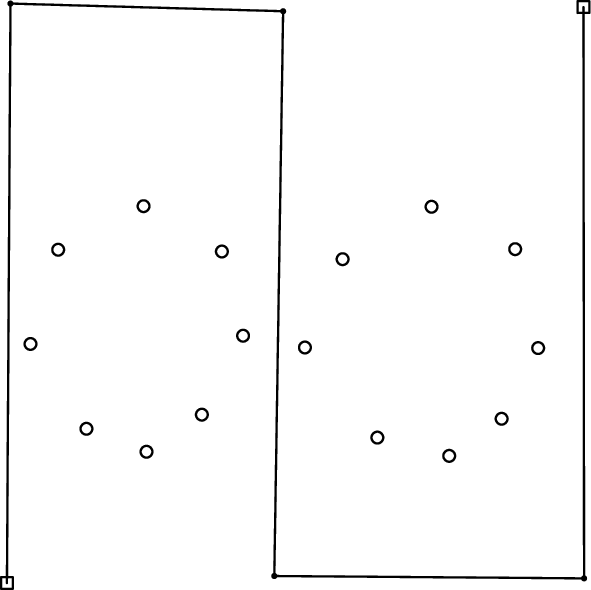
\includegraphics[width=0.5\textwidth]{image/ACMF1_1.png}
				
				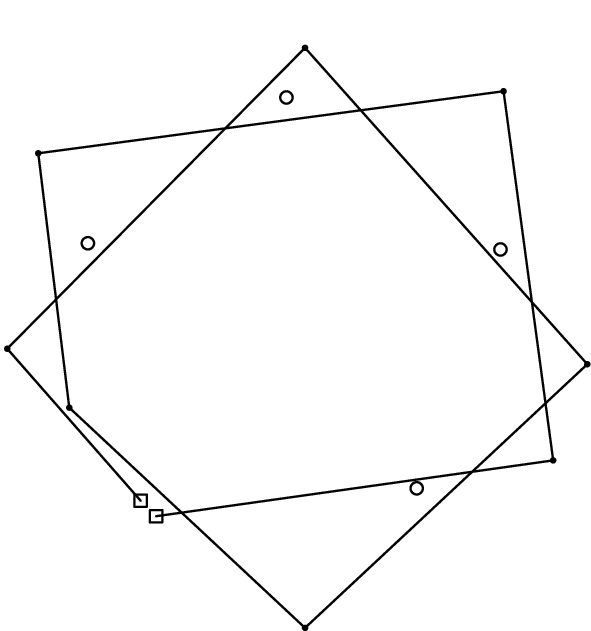
\includegraphics[width=0.5\textwidth]{image/ACMF2_1.png}
			\end{center}
		\end{column}
		\begin{column}{0.05\textwidth}
			\begin{center}
				$\Longrightarrow$
				\vskip 6em
				$\Longrightarrow$
			\end{center}
		\end{column}
		\begin{column}{0.475\textwidth}
			\begin{center}
				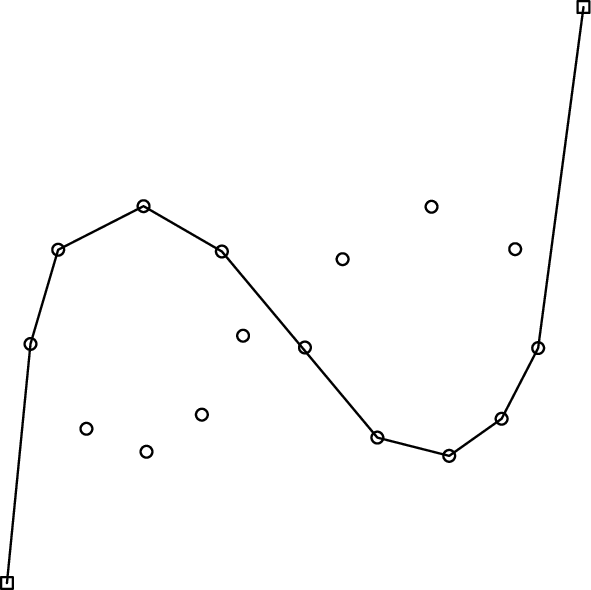
\includegraphics[width=0.5\textwidth]{image/ACMF1_2.png}
				
				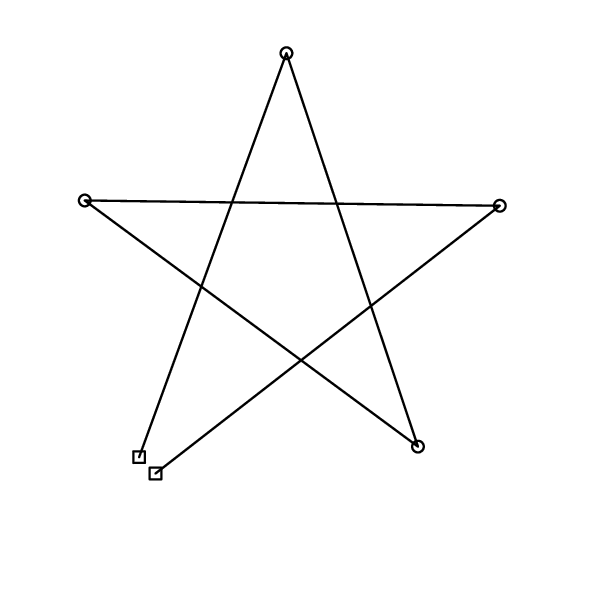
\includegraphics[width=0.5\textwidth]{image/ACMF2_2.png}
			\end{center}
		\end{column}
	\end{columns}
\end{qedframe}
\begin{qedframe}
	\frametitle{Tighten Up!}
	\begin{columns}
		\begin{column}{0.475\textwidth}
			\begin{center}
				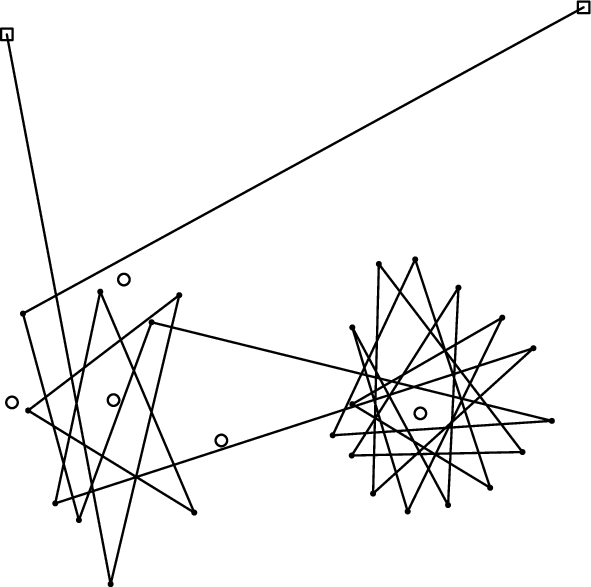
\includegraphics[width=0.7\textwidth]{image/ACMF3_1.png}
			\end{center}
		\end{column}
		\begin{column}{0.05\textwidth}
			\begin{center}
				$\Longrightarrow$
			\end{center}
		\end{column}
		\begin{column}{0.475\textwidth}
			\begin{center}
				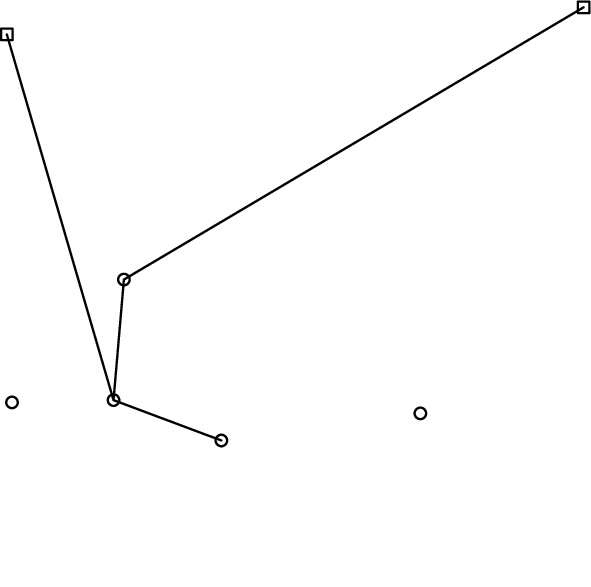
\includegraphics[width=0.7\textwidth]{image/ACMF3_2.png}
			\end{center}
		\end{column}
	\end{columns}
\end{qedframe}
\begin{qedframe}
	\frametitle{Tighten Up!}
	我们先看一道相对简单的题目:
	\begin{itemize}
		\item 平面上有一些固定的杆子。给定平面上一段闭合的绳圈,问能否将其收缩至无穷小的面积?\pause
	\end{itemize}
	\vskip 1em
	一个直观的想法是,如果有一个点在绳圈的``内部'',那么就无法收缩至无穷小,否则可以。判断内部可以求出点与每条边的有向角度之和,如果为0则不是内部。
\end{qedframe}
\begin{qedframe}
	\frametitle{Tighten Up!}
	但这个做法其实是错的,反例如下:
	\graph{ACMF4.png}{0.5}
\end{qedframe}
\begin{qedframe}
	\frametitle{Tighten Up!}
	正确做法如下:假设任意两点的横坐标都不同,作$n$条竖线穿过每个点,并对这$2n$条射线标号。我们记录绳圈穿过这些射线的顺序,比如下面的绳圈会对应序列
	\[0\rightarrow1\rightarrow2\rightarrow2\rightarrow1\rightarrow1\rightarrow2\rightarrow5\rightarrow1\rightarrow4\rightarrow5\rightarrow5\rightarrow1\rightarrow3\]
	\graph{ACMF5_1.png}{0.4}
\end{qedframe}
\begin{qedframe}
	\frametitle{Tighten Up!}
	而很显然,如果序列中出现了两个相邻且相同的数字,就意味着绳圈来回穿过了这条线,在将其``拉直''后肯定不会穿过。因此我们每次可以删去序列中两个相邻且相同的数字。对上面的序列处理完之后如下
	\[0\rightarrow1\rightarrow2\rightarrow5\rightarrow1\rightarrow4\rightarrow1\rightarrow3\]
	\graph{ACMF5_2.png}{0.4}
\end{qedframe}
\begin{qedframe}
	\frametitle{Tighten Up!}
	那对于这道题而言,我们只需判断能否通过这一操作将序列删空即可。
	
	我们将这一思路带回原题,同样对原题求出一个序列。我们现在要求的是,以给定的两点为端点,且满足这一序列的最短(因为被拉紧了)绳子长度。\pause
	
	这其实是一个DP问题。令$f[i]$表示绳子到序列第$i$位为止的长度,此时绳子的一段必然在序列这一位的射线对应的柱子上。我们枚举这一段绳子绕过的上一个节点是哪个,并判断是否可行。
	
	复杂度$O((nm)^2)$,因为理论上序列的长度可以达到$O(nm)$。
\end{qedframe}
\begin{qedframe}
	\frametitle{Tighten Up!}
	\begin{columns}
		\begin{column}{0.475\textwidth}
			\begin{center}
				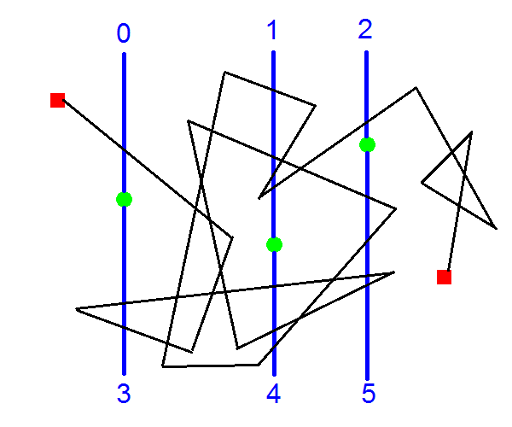
\includegraphics[width=0.9\textwidth]{image/ACMF6_1.png}
			\end{center}
		\end{column}
		\begin{column}{0.05\textwidth}
			\begin{center}
				$\Longrightarrow$
			\end{center}
		\end{column}
		\begin{column}{0.475\textwidth}
			\begin{center}
				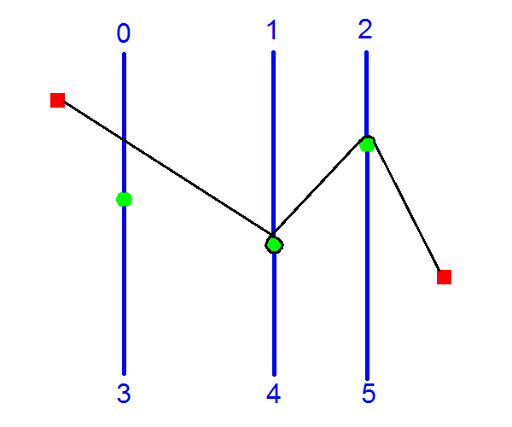
\includegraphics[width=0.9\textwidth]{image/ACMF6_2.png}
			\end{center}
		\end{column}
	\end{columns}
\end{qedframe}

\appendix
\section{}
\begin{frame}
	\frametitle{Fin.}
	\begin{center}
		\LARGE
		谢谢大家!欢迎课后交流。
	\end{center}
\end{frame}

\end{document}
